\documentclass[journal,twoside,web, 11pt]{ieeecolor}
\usepackage{generic}
\usepackage{cite}
\usepackage{amsmath,amssymb,amsfonts}
\usepackage{algorithmic}
\usepackage{graphicx}
\usepackage{textcomp}
\usepackage{microtype}
% \usepackage{setspace} % the text float beyond the blue edge on the top when using this.

\def\BibTeX{{\rm B\kern-.05em{\sc i\kern-.025em b}\kern-.08em
    T\kern-.1667em\lower.7ex\hbox{E}\kern-.125emX}}
\markboth{\journalname, VOL. XX, NO. XX, XXXX 2017}
{Author \MakeLowercase{\textit{et al.}}: Preparation of Papers for IEEE TRANSACTIONS and JOURNALS (February 2017)}

\begin{document}
\title{A nice title goes here}

\author{Chihcheng Hsieh, 
        Catarina Moreira,
        Chun Ouyang,
        Margot Brereton,
        Sandra Costa Sousa,
        Isabel Nobre Blanco, 
        Joaquim Jorge \IEEEmembership{Member, IEEE}, and
        Jo\~{a}o Madeiras Pereira
\thanks{This work was partially supported by Portuguese government national funds through FCT, Funda\c{c}\~{a}o para a Ci\^{e}ncia e a Tecnologia, under project UIDB/50021/2020.}
\thanks{C. Hsieh, C. Moreira, C. Ouyang and M. Brereton are with Queensland University of Technology, Brisbane Australia (e-mail: chihcheng.hsieh@hdr.qut.edu.au, \{pintomor,c.ouyang,m.brereton\}@qut.edu.au). }
\thanks{S.C. Costa, and I.B. Nobre are with Lus\'{i}adas Knowledge Centre, Portugal (e-mail: {sandra.costa.sousa,isabel.blanco.nobre}@lusiadas.pt).}
\thanks{J. Jorge and J.M. Pereira are with Instituto Superior T\'{e}cnico, University of Lisbon, Portugal (e-mail: jorgej@tecnico.ulisboa.pt, jap@inesc-id.pt).}}

\maketitle

% journal special issue: \url{https://www.embs.org/jbhi/special-issues-page/interpretable-deep-learning-idl-in-co-clinical-non-invasive-radiological-image/?fbclid=IwAR32n-Mi88Bhq3AIC134qXM-8AWu9YxsGfMVdDNz4aqKJMRGvsScvd0il84}
% according to the journal guidelines, the paper cannot have more than 200 words in the abstract and can't have more then 12 pages (with double space).

%%%%%%%%%%%%%%%%%%%%%% [TODO] %%%%%%%%%%%%%%%%%%%%%%
% [ ] - Write the result section.
% [ ] - Answer the questions in the abstract section.
%%%%%%%%%%%%%%%%%%%%%%%%%%%%%%%%%%%%%%%%%%%%%%%%%%%%

\begin{abstract}

% what is this about

% what you did

% why you did it

% how you did it

% what you found

\end{abstract}

\begin{IEEEkeywords}
%Enter key words or phrases in alphabetical  order, separated by commas. For a list of suggested keywords, send a blank  e-mail to keywords@ieee.org or visit \underline {http://www.ieee.org/organizations/pubs/ani\_prod/keywrd98.txt}
\end{IEEEkeywords}


\doublespacing
\section{Introduction} \label{sec:introduction}



\section{Related Work}
\subsection{Abnormality Detection}
\subsection{Multi-modal Learning}

\section{Multi-modal Learning Abnormality Detection}


\subsection{Datasets}
% Talk about What is MIMIC

% More detail about MIMIC-IV
The Medical Information Mart for Intensive Care (MIMIC) IV dataset \cite{Johnson2021MIMIC_IV} is sourced from two in-hospital database systems, a custom hospital wide EHR and an ICU specific clinical information system, in Beth Israel Deaconess Medical Center (BIDMC) between 2011 and 2019. The MIMIC-IV database is grouped into three modules, including \textit{core}, \textit{hosp} and \textit{icu}. The \textit{core} module contains patient tracking information for analysing MIMIC-IV, such as admissions, patients and transfers. The \textit{transfer} and the \textit{patients} tables required in our work. The transfer table allow us to link the CXR images to their specific stays in emergency department. And, the \textit{patients} table is one of the source of clinical data, which provides patients' gender and age. The \textit{hosp} module stores the hospital level data for patients derived from hospital wide electronic health record (EHR), including laboratory microbiology cultures, medication administration, hospital billing information, etc. At the last, the \textit{icu} module contains the patients' data when they stay in ICU, which includes their input (intravenous and fluid inputs) and output (urine and drainage) events.\\
\\

% Explain the relationship between MIMIC-IV, MIMIC-IV ED and MIMIC-CXR
Except the MIMIC-IV dataset we mentioned, there are two MIMIC-IV subsets, MIMIC-IV ED (Emergency Department) \cite{Johnson2021MIMIC_IV_ED} and MIMIC-CXR (Chest X-ray) \cite{Johnson2019MIMIC_CXR}, can be linked to MIMIC-IV dataset. The MIMIC-IV ED dataset was extracted from emergency department in the Beth Israel Deaconess Medical Center. It contains data for emergency department patients collected while they are in the ED. And, the \textit{triage} table in MIMIC-IV ED dataset is another source of clinical data providing the patients' health condition, such as \textit{temperature}, \textit{heart rate} and \textit{resprate}. MIMIC-CXR is another subset of MIMIC-IV consisting of 227,835 radiographic studies from BIDMC EHR between 2011 - 2016. This dataset contains radiology report and 377,110 radiographs used in the studies. In the original MIMIC-CXR dataset, the CXR images are provided in \textit{DICOM} format, which allows to adjust the exposure of radiograph to make a precise diagnosis. However, to train a machine learning model, the \textit{JPG} file is preferred. The MIMIC-CXR JPG dataset \cite{DJohnson2019MIMIC_CXR_JPG} made by the same author is then presented to facilitate the training process. The radiographs in MIMIC-CXR JPG dataset is the source of the Chest X-ray image input. Although, MIMIC-CXR already contains the radiologist report, which can be automatically transformed to labels through CheXpert \cite{Irvin2019Chexpert} or NegBio \cite{Yifan2017NegBio} labeler, it doesn't come with the bounding boxes annotating abnormalities; hence, the REFLACX dataset \cite{Lanfredi2021REFLACX} is considered. \\

To conduct the multimodal abnormality detection, we use the bounding ellipses provided in REFLACX dataset \cite{Lanfredi2021REFLACX} as the labels. The REFLACX dataset can be seen as a subset of MIMIC-IV, which provide extra data from different modalities, such as eye tracking data, abnormality bounding ellipses and time-stamped utterance. In this work, we use the abnormality bounding ellipses as labels for training object detection task. Other modalities from REFLACX will be considered in the future research. For the clinical dataset, we use patients data from MIMIC-IV and their health condition from MIMI-IV ED as the input of the multimodal learning framework. \\


The Figure \ref{fig: DataUsage} shows the overview of the data required in the training. The clinical data is extracted from MIMIC-IV Core \textit{patients} and MIMIC-IV ED \textit{triage} tables. The MIMIC-CXR JPG provides the CXR image in JPG format. And, these three data are considered the input of the model to generate corresponding predictions. At the last, the annotations from REFLACX dataset will be used as labels to calculate the loss for predictions. \\

\begin{figure*}[!h]
    \centering
    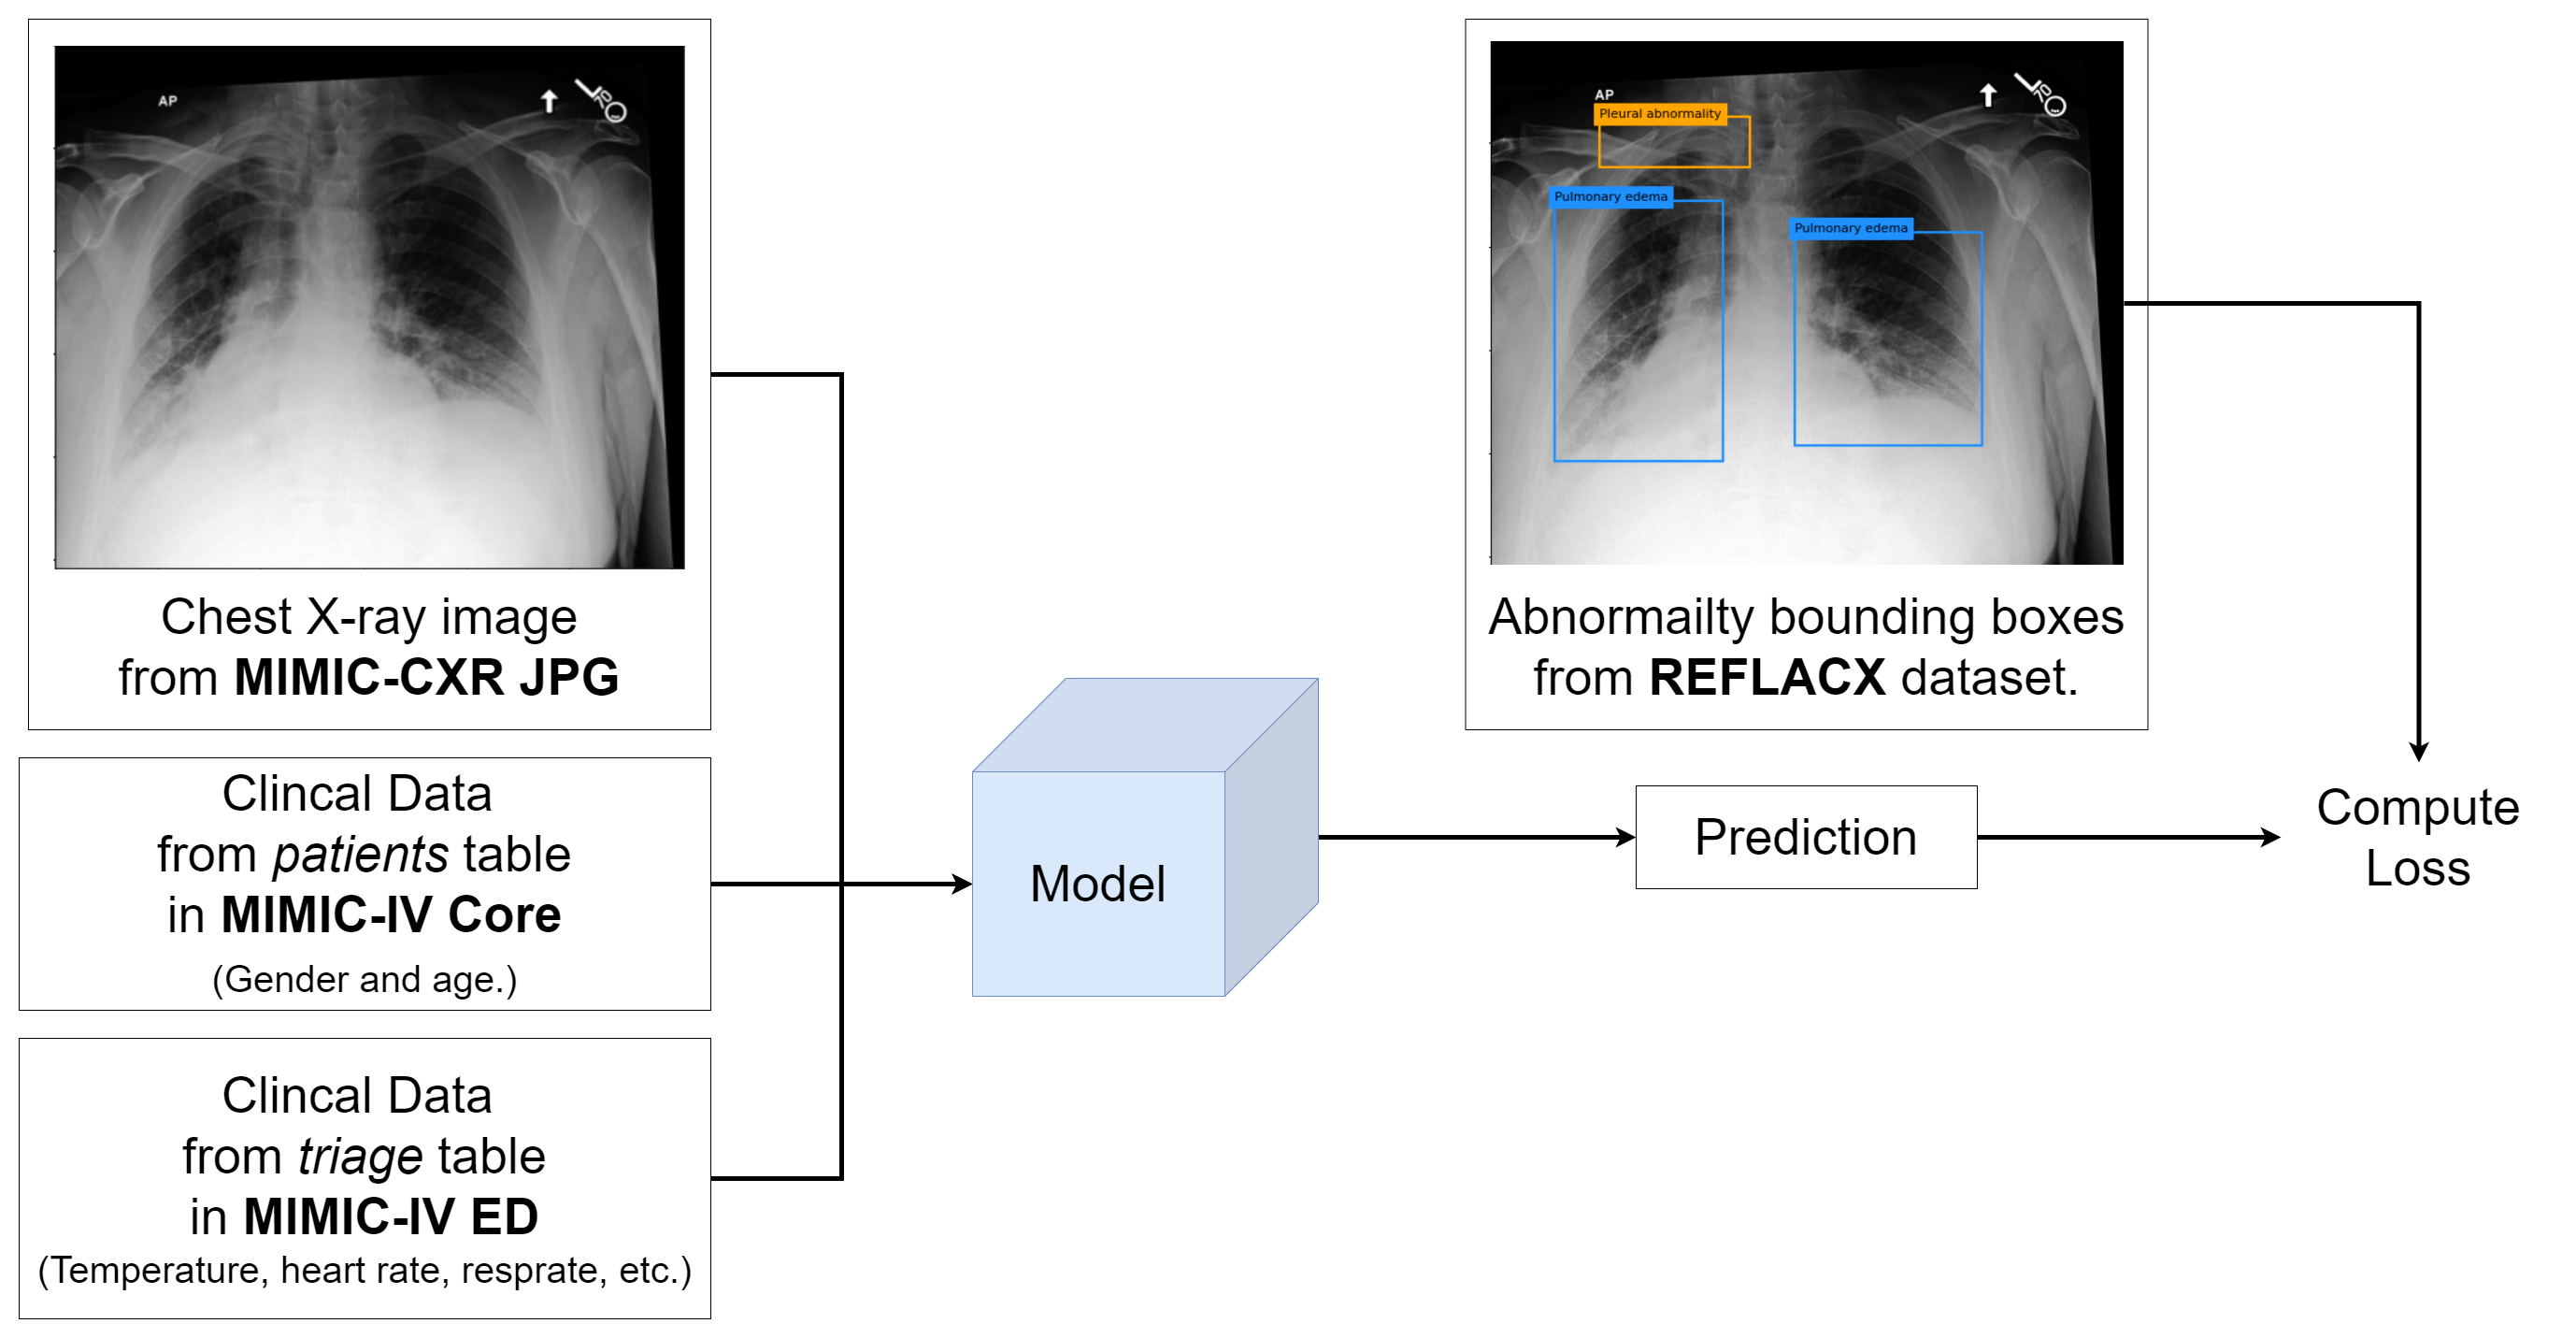
\includegraphics[width=\textwidth]{img/DataUsage.png}
    \centering
    \caption{Overview of the datasets used in training model.}
    \label{fig: DataUsage}
\end{figure*}


\begin{figure*}[!h]
    \centering
    \includegraphics[width=1\textwidth]{img/RepetitiveLabels.png}
    \caption{Repetitive labels in REFLACX dataset}
    \label{fig: repetitiveLables}
\end{figure*}

\subsection{Construction of REFLACX Multi-modal Learning dataset}

\textbf{\textit{Remove redundant labels}}: We found REFLACX dataset provide 2 versions of labels for radiologists to annotate lesions. As Figure \ref{fig: repetitiveLables} shows, the group of labels can be divided to V1 and V2. And, some of the labels exist in both V1 and V2. The REFLACX dataset contain 3052 cases in total. 2757 of them are annotated with V1 labels, and other 295 cases use V2 labels. To make the dataset concise and precise, we remap the redundant V2 labels to V1 labels. After the remapping, we ended up with 21 types of label (lesion). \\

\textbf{\textit{Retrieve patient's clinical data}}:  There are two tables in MIMIC-IV and MIMIC-IV ED contain the clinical data we desire. From MIMIC-IV Core patient table, we can retrieve patients' data, such as \textit{gender and age}. From MIMIC-IV ED triage table, we can extract the data related to patients' health condition, including \textit{temperature}, \textit{heart rate} and \textit{resprate}. To retrieve the data from both tables, we first need to identify the \textit{stay\_id} for each CXR image, which is an identifier which uniquely identifying a single emergency department stay for a single patient. According to our radiologists, data in these two tables are essential for them to make proper diagnosis. Although some free-text features are provided in \textit{triage} and \textit{patients} tables, we don't include them as input since it will introduce one extra sequential and unstructured modality, which our proposed architecture is hard to cooperate with.\\
\\

However, we encounter a version conflict in this stage, which results a significant data loss. Currently, two versions, 0.4v and 1.0v, of MIMIC-IV dataset are available on PhysioNet. At the 1.0v update, the \textit{id} for each patient is regenerated, which cause the incompatibility between 1.0v and 0.4v. Although we have the MIMIC-IV ED dataset updated to 1.0v, the MIMIC-CXR dataset has remained in 0.4 compatible version. As the result, we could only identify and retrieve clinical data for 670 cases with 590 unique CXR images in REFLACX dataset. \\

% Talk about that different annotations on the same CXR image. 
\begin{figure*}[!h]
    \centering
    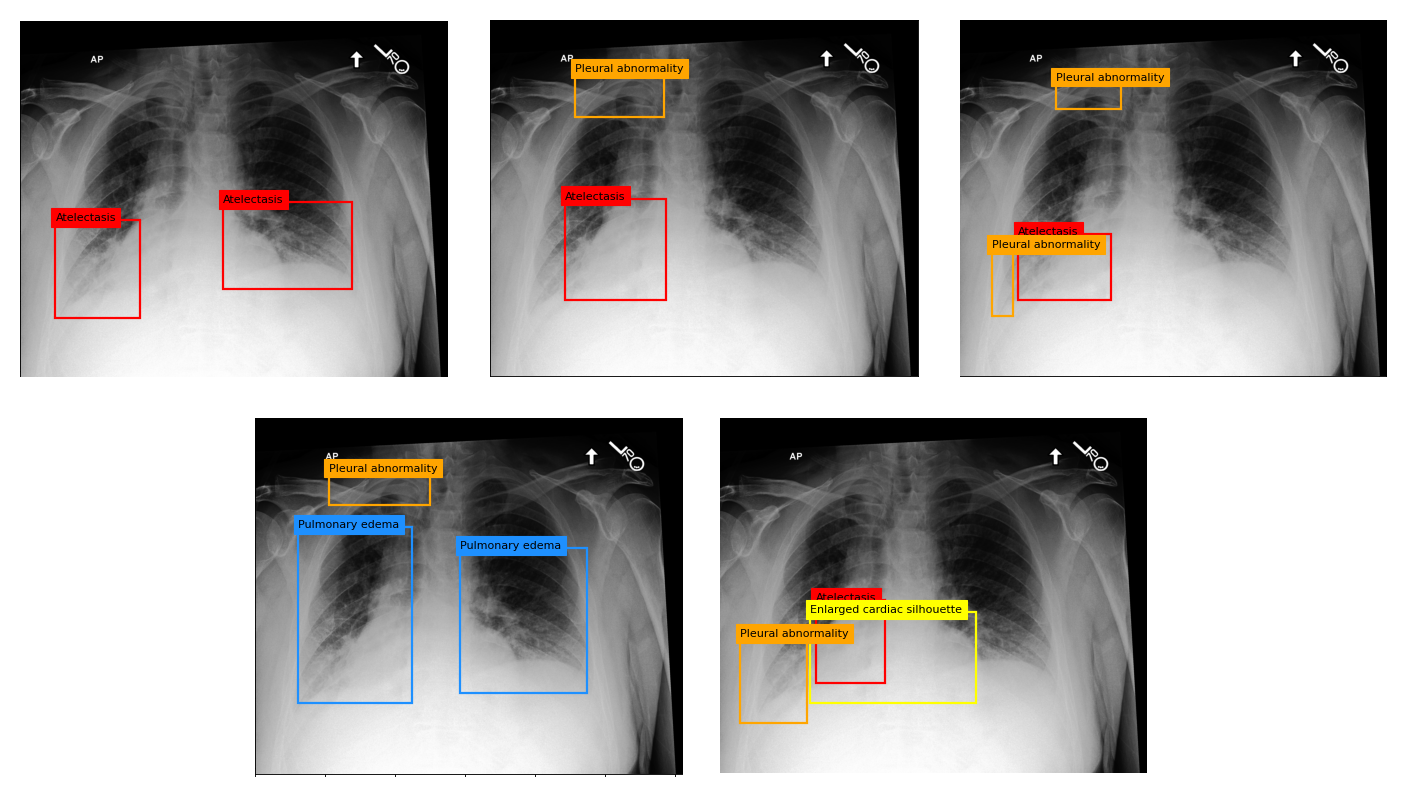
\includegraphics[width=\textwidth]{img/SameCXRAnnotatedByDifferenetRadiologsits.png}
    \caption{Same CXR image annotated by different radiologists in REFLACX dataset.}
    \label{fig: SameCXRAnnotatedByDifferenetRadiologsits}
\end{figure*}


\textbf{\textit{Uniquify CXR images}} : As demonstrated in Figure \ref{fig: SameCXRAnnotatedByDifferenetRadiologsits}, the same CXR image can be annotated by different radiologists in REFLACX dataset. And, the same figure also shows that the annotations are inconsistent across different radiologist, which may confuse the model as we expect the model to have different output while giving same input. To uniquify the CXR images, we put the annotations from different radiologists into single case, as shown at Figure \ref{fig: UniquifyCXR}.\\

\textbf{\textit{Top 5 with most occurrences}}: Some of the label doesn't have much occurrence; therefore, we decided to use 5 most frequent label, which can give model sufficient cases to learn. These top 5 labels are \textit{Enlarged cardiac silhouette, Atelectasis, Pleural abnormality, Consolidation and Pulmonary edema}. Patients with others disease except these top 5 disease will be considered as healthy patients without any lesion. \\ 

\textbf{\textit{Transform ellipses to boxes}}: The bounding ellipses indicating abnormalities (lesions) in REFLACX dataset will be transformed to bounding boxes to simplify the calculation on Intersection over Union ratio (IoU) and Intersection over the detected Bounding Box area ratio (IoBB). For each bounding ellipse in REFLACX dataset, they provide the maximum and minimum value in x and y axes, which can also be seen as the top left corner ($x_{min}, y_{min}$) and bottom right ($x_{max}, y_{max}$) of the bounding boxes.\\

\textbf{\textit{Split dataset}}: At the end, we split the dataset to train, validation and test dataset with portion of 70\%, 15\% and 15\% respectively, which means we have 413 cases for training the model. And, 88 and 89 cases for validating and testing purpose.\\

\begin{figure*}[!h]
    \centering
    \includegraphics[width=\textwidth]{img/UniquifyCXR.png}
    \caption{Uniquify annotations from different radiologists.}
    \label{fig: UniquifyCXR}
\end{figure*}

\subsection{Model Overview}

% See how Faster R-CNN describe their architecture.
Currently, there are countless models available to perform object detection. We first attempt to use Faster R-CNN \cite{Shaoqing2015FasterRCNN} as the architecture. However, this Faster R-CNN based model didn't give the stability and trainability we expect. We found another work \cite{Amit2019pneumonia} encountered the same problem while using Faster R-CNN model. They managed to solve this issue by transforming the bounding boxes to segmentation map and use it as another label to train a Mask R-CNN\cite{Kaiming2017MaskRCNN}. This strategy enable the model to learn from different tasks, which is considered as Multitask Learning \cite{Michael2020MultitaskLearning}. The Multitask Learning improves the data efficiency and the generalisation of the model. \\

We use Mask RCNN for uni-modal experiments. A brief overview of Mask RCNN model is shown in Figure \ref{fig: Uni-modal architecture}. The CXR images are firstly passed into a pretrained Convolutional Neural Network (CNN), which can be ResNet50\cite{Kaiming2015ResNet}, MobileNet\cite{Andrew2017MobileNets} or other CNN models that can extract features maps from image. For the demonstration purpose, MobileNet is used in the figure; however, in the later experiments, the a more complex ResNet50 with Feature Pyramid Networks (FPN) \cite{Tsung2016FPN} is used since it provide a better performance. After the features maps are obtained, they will be passed into another Region Proposal Network (RPN), which is another CNN model responsible for generating rougher bounding boxes coordinates (proposals). According to the bounding boxes from RPN, the model then retrieve related area in the features maps as the input for the final classifier to determine the finer bounding boxes coordinates, segmentation map (mask) and the lesions (classes) inside bounding boxes.\\

For the multimodal experiments, the proposed model is shown in Figure \ref{fig: Multi-modal architecture}. Same as the uni-modal architecture, the MobileNet in the figure will be replace by ResNet50 with FPN to gain better performance. In order to fuse the clinical data with CXR image, we first need to transform them to the same dimensions. The cetegorical clinical data is first embedded into vectors then concatenate with numerical clinical data. After the concatenation, we see the concatenated vector as a 1 pixel image and use several decovolutional (transposed convolution) layers \cite{Zeiler2010Deconv} to upsample and spatialise it until it match the size of \textit{Image Feature Maps}. Once we have same dimension \textit{Image Feature Maps} and \textit{Clinical Feature Maps}, we apply the fusion operation, which is simply several layers of CNN, to blend the information from different modalities. After the fusion phase, the rest of the architecture are identical to the uni-modal architecture.\\

\begin{figure*}[!h]
    \centering
    
\includegraphics[width=\textwidth]{img/FaseterRCNN-MobileNet simplified.png}
    \caption{Multi-modal architecture.}
    \label{fig: Multi-modal architecture}
\end{figure*}


\begin{figure*}[!h]
    \centering
    \includegraphics[width=\textwidth]{img/Multimodal Faster R-CNN MobileNet simplified.png}
    \caption{Uni-modal architecture.}
    \label{fig: Uni-modal architecture}
\end{figure*}

\subsection{Spatialise Clinical Data}
talking about how we manage to transform the clinical (tabular) data to 3D tensor (spatial data).

\subsection{Fusion} 
talking about the fusion strategy we use, talking about the layer of fusion depth and the residule method we provide.

\section{Experiments}


\subsection{Setup}

The most common backbone used with Mask R-CNN is ResNet \cite{}. However, we have a relatively smaller dataset. Therefore, MobileNet V3 is chosen to be the backbone of Mask R-CNN model, which contains only around 1M trainable parameters while the pretrained ResNet18 and ResNet50 have 11M and 23M trainable parameters respectively. \\

When the pretrained backbone is used with the CXR model, we observed the model to converge faster and result in overfitting, as Figure \ref{fig: overfitting} shown. To mitigate the overfitting, we applied dropout, L2 regularization, early stop strategy, model size reduction and learning rate scheduler. With these solutions applied to the model, we not only has a smaller model without overfitting issue but also gain a small performance improvement. And, the Figure \ref{overfitting_solution_applied} shows a more stabilised and optimum fitting training progress.\\

Because of the additional clinical and fusion layers for processing the clinical input and fusing image and clinical features, the clinical model is 1.21 times larger than the model using CXR images only. The number of trainable parameters and other hyper parameters are shown in the Table \ref{tab:hpyer-params}. Although the CXR + clinical model is a larger model, it doesn't have overfitting issue since the clinical NN used and the fusion operations are untrained, which promote under-fitting in the beginning of the training. And, this is also the reason for training CXR + clinical model for 100 more epochs to ensure the validation performance won't further improve.\\

In this experiment, the early stop strategy is used to capture the model when it reach its best performance on the validation set, which gives us a better balance between performance and generalization. The CXR model reached its best validation performance at epoch 30, while the CXR + clinical model has its best performance at epoch 111.\\

As the Table \ref{tab:eval_training} shown, the CXR model perform better on the training set; however, it fail to generalise to validation and test sets in Table \ref{tab:eval_validation} and Table  \ref{tab:eval_test} respectively.\\


\begin{table}[h!]
    \centering
    \caption{Training hyper-parameters.}
    \begin{tabular}{|l|r|r|}
    %\multicolumn{3}{|c|}{Parameters}\\
    \hline
    Parameters & CXR Model & CXR + Clinical Model \\
    \hline
        Model size &  1,040,729 & 1,223,303  \\
        Learning rate &  0.01 & 0.001 \\
        Epochs & 100 & 200 \\
        Batch size & 4 & 4  \\
        Weight decay (L2) & 0.001  & 0.001\\
    \hline
    \end{tabular}
    \label{tab:hpyer-params}
\end{table}

% \begin{table}[h!]
%     \centering
%     \caption{Model performance on different datasets.}
%     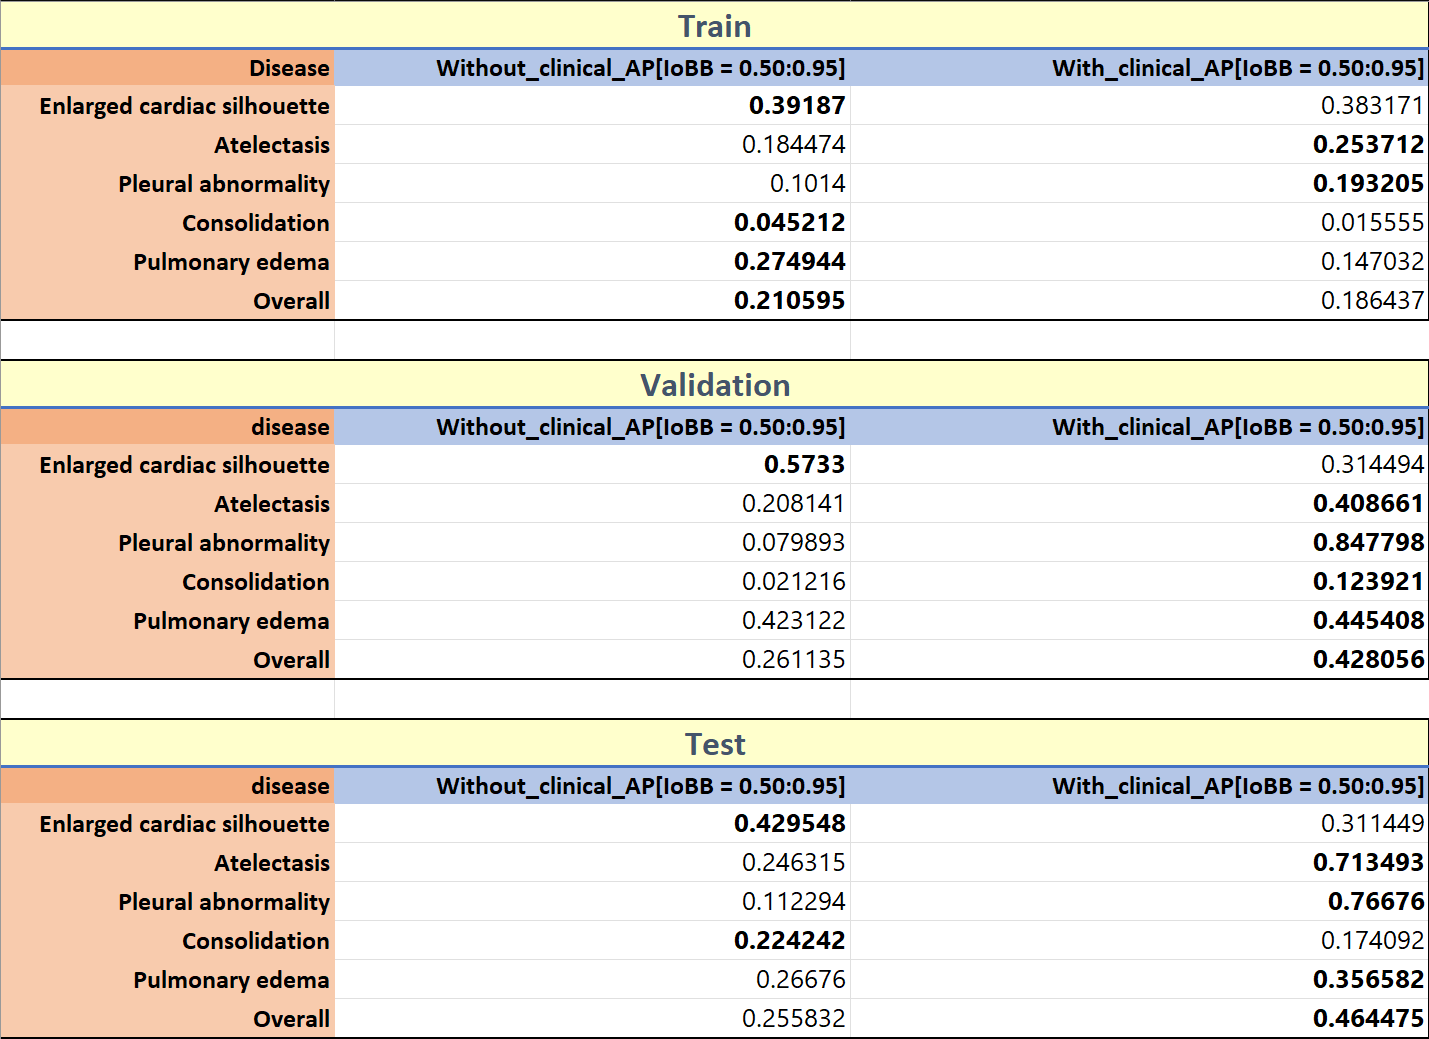
\includegraphics[width=\textwidth]{img/eval_all.png}
%     \label{tab:training_params}
% \end{table}



\begin{figure*}[!h]
    \centering
    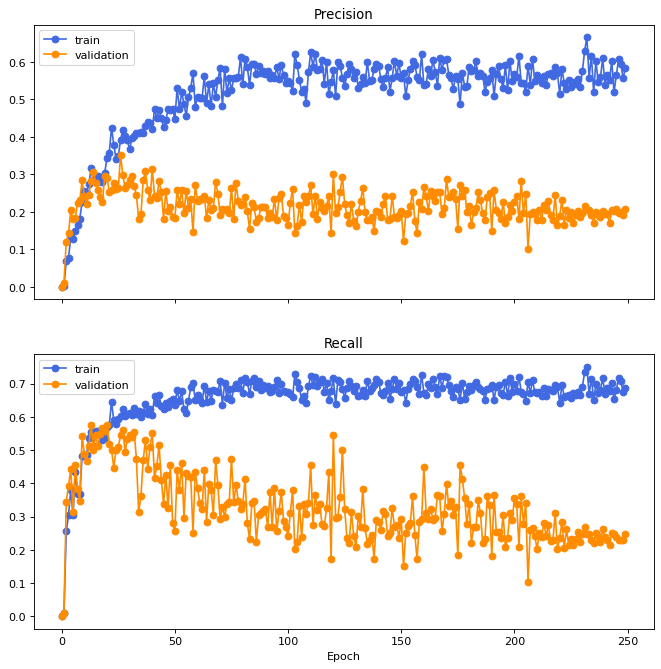
\includegraphics[width=\textwidth]{img/overfitting.png}
    \caption{Training progress shows overfitting issue on CXR model.}
    \label{fig: overfitting}
\end{figure*}

\begin{figure*}[!h]
    \centering
    \includegraphics[width=\textwidth]{img/overfitting_solution_applied.png}
    \caption{CXR model's training progress after overfitting solution applied.}
    \label{fig: overfitting_solution_applied}
\end{figure*}

\begin{figure*}[!h]
    \centering
    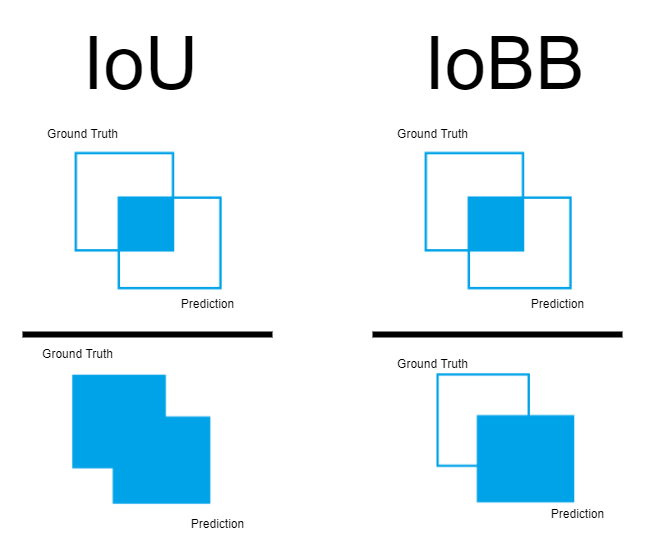
\includegraphics[width=.8\textwidth]{img/iou_iobb.png}
    \caption{Iou and IoBB}
    \label{fig: iou_iobb}
\end{figure*}

\begin{figure*}[!h]
    \centering
    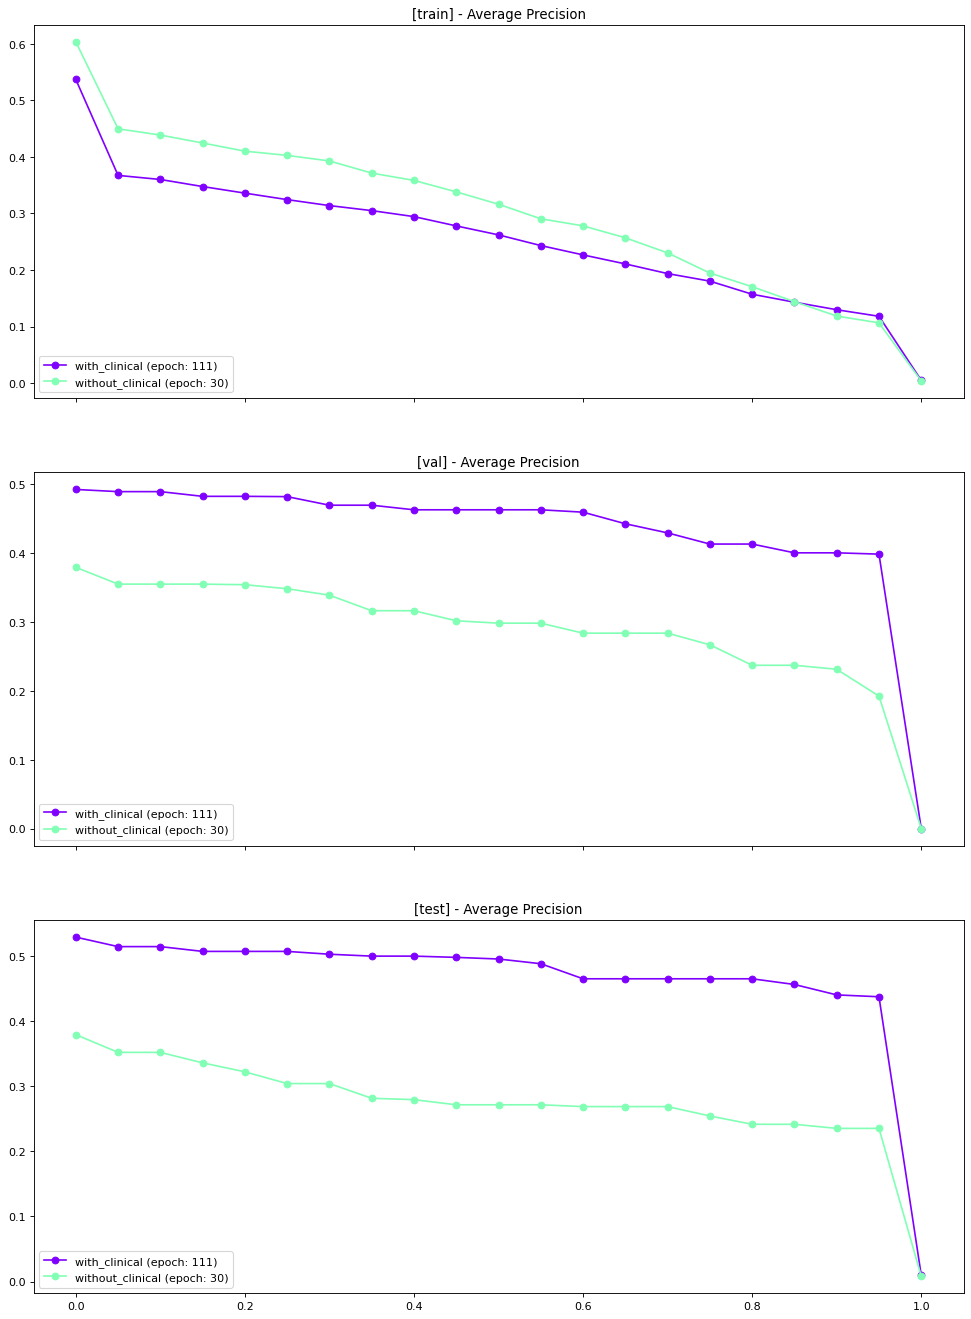
\includegraphics[width=\textwidth]{img/performance.png}
    \caption{Model performance on different IoBB thresholds.}
    \label{fig: performance}
\end{figure*}

\subsection{Main Results}

% Findings:
% 1. Adding the clinical data improves the model performance by 
% 2. Adding the clinical data improves the generalization.
% 3. The CXR model has overfitting issue, but the CXR + clinical model has the underfitting issue.
% 4. 

%%%%%%%% Training Eval Table %%%%%%%% 
\begin{table*}[]
\centering
\caption{Evaluation on training set. (Score threshold = 0.05)}
\label{tab:eval_training}
\begin{tabular}{lrrrr}
\hline
\textbf{Disease}            & \multicolumn{2}{c}{\textbf{CXR Model}}                                                                                                                                                            & \multicolumn{2}{c}{\textbf{CXR+Clinical Model}}                                                                                                                                                   \\ \hline
                            & \multicolumn{1}{c}{\textbf{\begin{tabular}[c]{@{}c@{}}AP\\ @{[}IoBB=0.50:0.95{]}\end{tabular}}} & \multicolumn{1}{c}{\textbf{\begin{tabular}[c]{@{}c@{}}AR\\ @{[}IoBB=0.50:0.95{]}\end{tabular}}} & \multicolumn{1}{c}{\textbf{\begin{tabular}[c]{@{}c@{}}AP\\ @{[}IoBB=0.50:0.95{]}\end{tabular}}} & \multicolumn{1}{c}{\textbf{\begin{tabular}[c]{@{}c@{}}AR\\ @{[}IoBB=0.50:0.95{]}\end{tabular}}} \\ \hline
Enlarged cardiac silhouette & \textbf{0.39187}                                                                                & 0.573387                                                                                        & 0.383171                                                                                        & \textbf{0.658065}                                                                               \\
Atelectasis                 & 0.184474                                                                                        & 0.42284                                                                                         & \textbf{0.253712}                                                                               & \textbf{0.526543}                                                                               \\
Pleural abnormality         & 0.1014                                                                                          & 0.354762                                                                                        & \textbf{0.193205}                                                                               & \textbf{0.416667}                                                                               \\
Consolidation               & \textbf{0.045212}                                                                               & \textbf{0.279104}                                                                               & 0.015555                                                                                        & 0.177612                                                                                        \\
Pulmonary edema             & \textbf{0.274944}                                                                               & \textbf{0.587129}                                                                               & 0.147032                                                                                        & 0.466337                                                                                        \\ \hline
\textbf{Overall}            & \textbf{0.210595}                                                                               & 0.455672                                                                                        & 0.186437                                                                                        & \textbf{0.463208}                                                                               \\ \hline
\end{tabular}
\end{table*}


%%%%%%%% Validation Eval Table %%%%%%%% 
\begin{table*}[]
\centering
\caption{Evaluation on validation set. (Score threshold = 0.05)}
\label{tab:eval_validation}
\begin{tabular}{lrrrr}
\hline
\textbf{Disease}            & \multicolumn{2}{c}{\textbf{CXR Model}}                                                                                                                                                            & \multicolumn{2}{c}{\textbf{CXR+Clinical Model}}                                                                                                                                                   \\ \hline
                            & \multicolumn{1}{c}{\textbf{\begin{tabular}[c]{@{}c@{}}AP\\ @{[}IoBB=0.50:0.95{]}\end{tabular}}} & \multicolumn{1}{c}{\textbf{\begin{tabular}[c]{@{}c@{}}AR\\ @{[}IoBB=0.50:0.95{]}\end{tabular}}} & \multicolumn{1}{c}{\textbf{\begin{tabular}[c]{@{}c@{}}AP\\ @{[}IoBB=0.50:0.95{]}\end{tabular}}} & \multicolumn{1}{c}{\textbf{\begin{tabular}[c]{@{}c@{}}AR\\ @{[}IoBB=0.50:0.95{]}\end{tabular}}} \\ \hline
Enlarged cardiac silhouette & \textbf{0.5733}                                                                                 & \textbf{0.854545}                                                                               & 0.314494                                                                                        & 0.672727                                                                                        \\
Atelectasis                 & 0.208141                                                                                        & 0.444444                                                                                        & \textbf{0.408661}                                                                               & \textbf{0.65}                                                                                   \\
Pleural abnormality         & 0.079893                                                                                        & 0.364286                                                                                        & \textbf{0.847798}                                                                               & \textbf{0.928571}                                                                               \\
Consolidation               & 0.021216                                                                                        & 0.142857                                                                                        & \textbf{0.123921}                                                                               & \textbf{0.428571}                                                                               \\
Pulmonary edema             & 0.423122                                                                                        & 0.653846                                                                                        & \textbf{0.445408}                                                                               & \textbf{0.7}                                                                                    \\ \hline
\textbf{Overall}            & 0.261135                                                                                        & 0.491996                                                                                        & \textbf{0.428056}                                                                               & \textbf{0.675974}                                                                               \\ \hline
\end{tabular}
\end{table*}


%%%%%%%% Test Eval Table %%%%%%%% 
\begin{table*}[]
\centering
\caption{Evaluation on test set. (Score threshold = 0.05)}
\label{tab:eval_test}
\begin{tabular}{lrrrr}
\hline
\textbf{Disease}            & \multicolumn{2}{c}{\textbf{CXR Model}}                                                                                                                                                            & \multicolumn{2}{c}{\textbf{CXR+Clinical Model}}                                                                                                                                                   \\ \hline
                            & \multicolumn{1}{c}{\textbf{\begin{tabular}[c]{@{}c@{}}AP\\ @{[}IoBB=0.50:0.95{]}\end{tabular}}} & \multicolumn{1}{c}{\textbf{\begin{tabular}[c]{@{}c@{}}AR\\ @{[}IoBB=0.50:0.95{]}\end{tabular}}} & \multicolumn{1}{c}{\textbf{\begin{tabular}[c]{@{}c@{}}AP\\ @{[}IoBB=0.50:0.95{]}\end{tabular}}} & \multicolumn{1}{c}{\textbf{\begin{tabular}[c]{@{}c@{}}AR\\ @{[}IoBB=0.50:0.95{]}\end{tabular}}} \\ \hline
Enlarged cardiac silhouette & \textbf{0.429548}                                                                               & 0.531579                                                                                        & 0.311449                                                                                        & \textbf{0.552632}                                                                               \\
Atelectasis                 & 0.246315                                                                                        & 0.428571                                                                                        & \textbf{0.713493}                                                                               & \textbf{0.857143}                                                                               \\
Pleural abnormality         & 0.112294                                                                                        & 0.25                                                                                            & \textbf{0.76676}                                                                                & \textbf{0.8125}                                                                                 \\
Consolidation               & \textbf{0.224242}                                                                               & 0.325                                                                                           & 0.174092                                                                               & \textbf{0.375}                                                                                  \\
Pulmonary edema             & 0.26676                                                                                         & 0.5625                                                                                          & \textbf{0.356582}                                                                               & \textbf{0.625}                                                                                  \\ \hline
\textbf{Overall}            & 0.255832                                                                                        & 0.41953                                                                                         & \textbf{0.464475}                                                                               & \textbf{0.644455}                                                                               \\ \hline
\end{tabular}
\end{table*}


\section{Conclusion}
A conclusion section is not required. Although a conclusion may review the 
main points of the paper, do not replicate the abstract as the conclusion. A 
conclusion might elaborate on the importance of the work or suggest 
applications and extensions. 

\appendices

% Author photographs,  color, and grayscale figures should be at least 300dpi. Line art, including  tables should be a minimum of 600dpi.
% we accept files in the following formats: .EPS/.PDF/.PS. All 

Appendixes, if needed, appear before the acknowledgment.

\bibliographystyle{IEEEtran}
\bibliography{refs}

\section*{Acknowledgment}

\section*{References}


\end{document}

%%%%%%%%%%%%%%% Instructinos from IEEE %%%%%%%%%%%%%%%

%\subsection{Equations}
%Number equations consecutively with equation numbers in parentheses flush 
%with the right margin, as in \eqref{eq}. To make your equations more 
%compact, you may use the solidus (~/~), the exp function, or appropriate 
%exponents. Use parentheses to avoid ambiguities in denominators. Punctuate 
%equations when they are part of a sentence, as in
%\begin{equation}E=mc^2.\label{eq}\end{equation}
% Refer to ``\eqref{eq},'' not ``Eq. \eqref{eq}''  or ``equation \eqref{eq},'' except at the beginning of a sentence: ``Equation \eqref{eq}  is $\ldots$